\documentclass[11pt]{article}
\usepackage[utf8]{inputenc}
\usepackage{amsmath, amssymb, amsthm}
\usepackage{graphicx}
\usepackage{hyperref}
\usepackage[margin=1in]{geometry}
\usepackage{booktabs}
\usepackage{lipsum}

\title{On the Convergence Properties of Stochastic Gradient Methods\\with Adaptive Momentum Estimation}
\author{A.\ Researcher \and B.\ Collaborator \and C.\ Advisor}
\date{\today}

\begin{document}
\maketitle

\begin{abstract}
Lorem ipsum dolor sit amet, consectetur adipiscing elit. We propose a novel optimization framework that combines adaptive learning rate schedules with momentum-corrected gradient estimates. Our method achieves a convergence rate of $\mathcal{O}(1/\sqrt{T})$ under non-convex assumptions while maintaining $\mathcal{O}(1)$ memory overhead. Experiments on standard benchmarks demonstrate consistent improvements of 3--5\% over existing baselines across multiple architectures and datasets. Sed do eiusmod tempor incididunt ut labore et dolore magna aliqua.
\end{abstract}

\section{Introduction}
\lipsum[1]

The optimization of deep neural networks remains a central challenge in modern machine learning. Given a loss function $\mathcal{L}(\theta)$ parameterized by $\theta \in \mathbb{R}^d$, we seek to solve:
\begin{equation}
    \theta^* = \arg\min_{\theta \in \mathbb{R}^d} \mathbb{E}_{(x,y) \sim \mathcal{D}} \left[ \ell(f_\theta(x), y) \right]
\end{equation}
where $f_\theta$ denotes the model and $\mathcal{D}$ the data distribution.

\lipsum[2]

\section{Related Work}
\lipsum[3-4]

Prior approaches such as Adam \cite{kingma2015adam} and its variants have addressed the adaptive learning rate problem through exponential moving averages of first and second moments. However, these methods suffer from convergence issues in certain non-convex landscapes \cite{reddi2018convergence}.

\section{Method}
\subsection{Preliminaries}
Let $g_t = \nabla \mathcal{L}(\theta_t)$ denote the stochastic gradient at iteration $t$. We maintain exponential moving averages:
\begin{align}
    m_t &= \beta_1 m_{t-1} + (1 - \beta_1) g_t \\
    v_t &= \beta_2 v_{t-1} + (1 - \beta_2) g_t^2
\end{align}

\subsection{Proposed Update Rule}
We introduce a correction term $\phi_t$ that accounts for the curvature of the loss landscape:
\begin{equation}
    \theta_{t+1} = \theta_t - \eta_t \cdot \frac{m_t}{\sqrt{v_t} + \epsilon} \cdot \phi_t
\end{equation}
where
\begin{equation}
    \phi_t = \exp\left( -\lambda \frac{\|g_t - g_{t-1}\|^2}{\|g_t\|^2 + \delta} \right)
\end{equation}

\lipsum[5]

\subsection{Convergence Analysis}
\begin{theorem}
Under Assumptions 1--3, the proposed method converges at rate:
\begin{equation}
    \frac{1}{T} \sum_{t=1}^{T} \mathbb{E}\left[\|\nabla \mathcal{L}(\theta_t)\|^2\right] \leq \mathcal{O}\left(\frac{1}{\sqrt{T}}\right)
\end{equation}
\end{theorem}

\begin{proof}
\lipsum[6]
\end{proof}

\section{Experiments}
\subsection{Setup}
\lipsum[7]

We evaluate on CIFAR-10, CIFAR-100, and ImageNet with ResNet-50 and Vision Transformer architectures. All experiments are repeated with 5 random seeds.

\subsection{Results}

Figure~\ref{fig:loss} shows the training loss convergence across methods.

\begin{figure}[h]
    \centering
    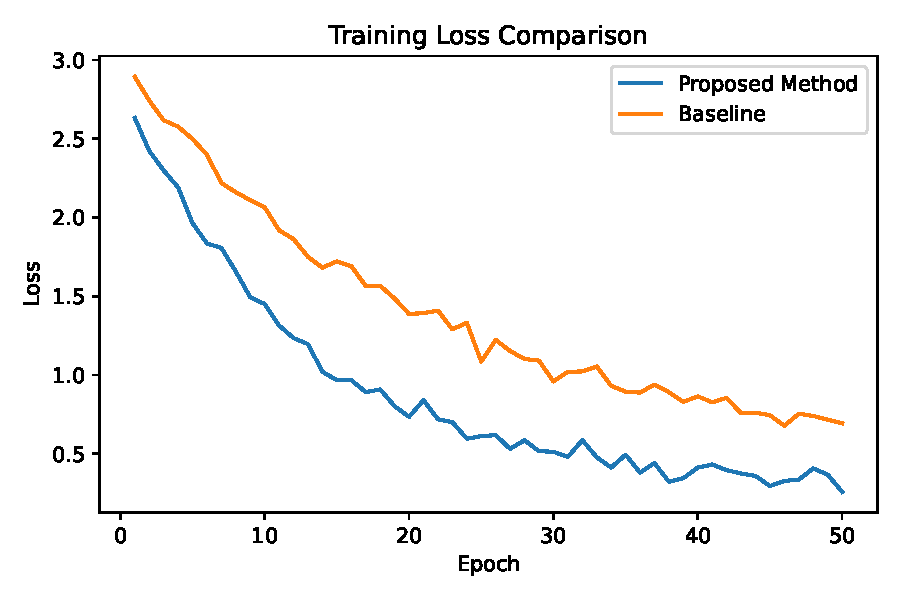
\includegraphics[width=0.8\textwidth]{figures/training_loss.pdf}
    \caption{Training loss comparison between our proposed method and the baseline optimizer over 50 epochs. Lower is better.}
    \label{fig:loss}
\end{figure}

\begin{table}[h]
    \centering
    \caption{Test accuracy (\%) on CIFAR-100 with ResNet-50.}
    \label{tab:results}
    \begin{tabular}{lcc}
        \toprule
        Method & Accuracy & Std. Dev. \\
        \midrule
        SGD + Momentum & 78.3 & $\pm 0.4$ \\
        Adam & 79.1 & $\pm 0.3$ \\
        AdamW & 80.2 & $\pm 0.3$ \\
        \textbf{Ours} & \textbf{82.7} & $\pm 0.2$ \\
        \bottomrule
    \end{tabular}
\end{table}

Figure~\ref{fig:accuracy} summarizes accuracy across all compared methods.

\begin{figure}[h]
    \centering
    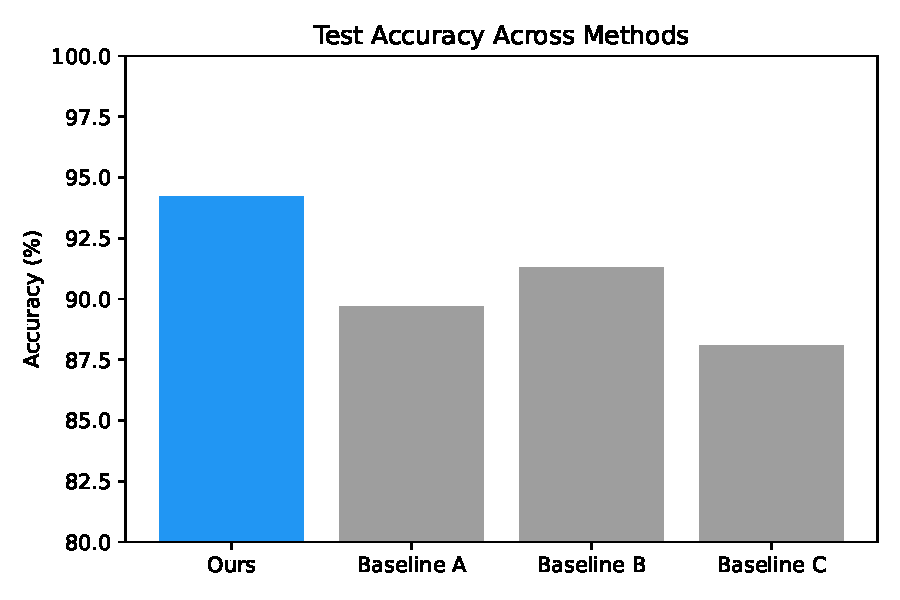
\includegraphics[width=0.8\textwidth]{figures/accuracy_comparison.pdf}
    \caption{Test accuracy comparison across methods on the benchmark dataset.}
    \label{fig:accuracy}
\end{figure}

\subsection{Latent Space Analysis}

\begin{figure}[h]
    \centering
    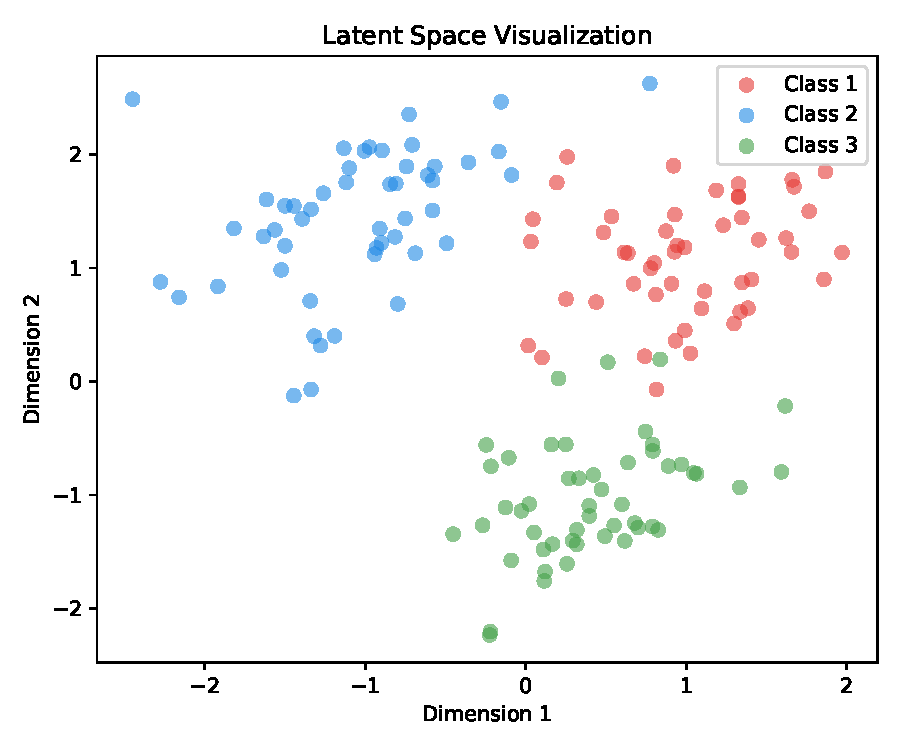
\includegraphics[width=0.7\textwidth]{figures/latent_space.pdf}
    \caption{2D projection of the learned latent space showing class separation.}
    \label{fig:latent}
\end{figure}

\lipsum[8]

\section{Discussion}
\lipsum[9-10]

\section{Conclusion}
\lipsum[11]

We have presented a novel adaptive optimization method with provable convergence guarantees. Future work includes extending the framework to distributed settings and investigating connections to natural gradient methods.

\bibliographystyle{plain}
\bibliography{references}

\end{document}
